\documentclass[12pt]{article}
\usepackage[labelfont=bf]{caption}
\usepackage{lmodern}
\usepackage{graphicx}
\usepackage{multirow}
\usepackage{booktabs}
\usepackage{newfloat}
\usepackage[flushleft]{threeparttable}
\usepackage{parskip}
\usepackage[
  backend=bibtex,
  style=numeric,
  sorting=none,
  doi=true,
  url=false,
  citestyle=numeric-comp
]{biblatex}

\AtEveryBibitem{%
  \clearlist{language}%
  }
\setlength\bibitemsep{\baselineskip}

\usepackage{cmbright}
\usepackage{sansmath}
\sansmath
\usepackage[scaled]{helvet}
\renewcommand\familydefault{\sfdefault}
\usepackage[math]{blindtext}

\usepackage[T1]{fontenc}

\bibliography{references.bib}
\usepackage{doi}
\usepackage{authblk}

\DeclareFloatingEnvironment[name={Figure}]{suppfigure}
\usepackage{amssymb,amsmath}
\usepackage[margin=2cm]{geometry}
\graphicspath{ {../Plots/FinalFigures/} }
\usepackage{lineno}
\usepackage{ifxetex,ifluatex}
\usepackage{fixltx2e} % provides \textsubscript
\ifnum 0\ifxetex 1\fi\ifluatex 1\fi=0 % if pdftex
  \usepackage[T1]{fontenc}
  \usepackage[utf8]{inputenc}
\else % if luatex or xelatex
  \ifxetex
    \usepackage{mathspec}
  \else
    \usepackage{fontspec}
  \fi
  \defaultfontfeatures{Ligatures=TeX,Scale=MatchLowercase}
\fi
% use upquote if available, for straight quotes in verbatim environments
\IfFileExists{upquote.sty}{\usepackage{upquote}}{}
% use microtype if available
\IfFileExists{microtype.sty}{%
\usepackage{microtype}
\UseMicrotypeSet[protrusion]{basicmath} % disable protrusion for tt fonts
}{}
\usepackage{hyperref}
\hypersetup{unicode=true,
            pdfborder={0 0 0},
            breaklinks=true,
            colorlinks=true,
            citecolor=blue
}
\urlstyle{same}  % don't use monospace font for urls
\IfFileExists{parskip.sty}{%
\usepackage{parskip}
}{% else
\setlength{\parindent}{0pt}
\setlength{\parskip}{6pt plus 2pt minus 1pt}
}
\setlength{\emergencystretch}{3em}  % prevent overfull lines
\providecommand{\tightlist}{%
  \setlength{\itemsep}{0pt}\setlength{\parskip}{0pt}}
\setcounter{secnumdepth}{0}
% Redefines (sub)paragraphs to behave more like sections
\ifx\paragraph\undefined\else
\let\oldparagraph\paragraph
\renewcommand{\paragraph}[1]{\oldparagraph{#1}\mbox{}}
\fi
\ifx\subparagraph\undefined\else
\let\oldsubparagraph\subparagraph
\renewcommand{\subparagraph}[1]{\oldsubparagraph{#1}\mbox{}}
\fi

\renewcommand\Authfont{\fontsize{13}{14.4}\selectfont}
\renewcommand\Affilfont{\fontsize{10}{10.8}\selectfont}

\date{}

\begin{document}

\title{Population scale mapping of transposable element diversity reveals links to gene regulation and epigenomic variation}

\author[1]{Tim Stuart}
\author[2]{Steven R. Eichten}
\author[1]{Jonathan Cahn}
\author[1]{Yuliya Karpievitch}
\author[2]{Justin Borevitz}
\author[1]{Ryan Lister}
\affil[1]{ARC Centre of Excellence in Plant Energy Biology, The University of
Western Australia, Perth, Australia}
\affil[2]{ARC Centre of Excellence in Plant Energy Biology, The Australian
National University, Canberra, Australia}

\renewcommand\Authands{ and }

\maketitle

Corresponding author: Ryan Lister \href{mailto:ryan.lister@uwa.edu.au}{ryan.lister@uwa.edu.au} \\

\textbf{Author ORCID IDs:}

0000-0002-3044-0897 (TS)

0000-0003-2268-395X (SRE)

0000-0002-5006-741X (JC)

0000-0001-6637-7239 (RL)


\linenumbers

\section{Abstract}

Variation in the presence or absence of transposable elements (TEs) is
a major source of genetic variation between individuals. Here, we
identified 23,095 TE presence/absence variants between 216 Arabidopsis
accessions. Most TE variants were rare, and we find a burden of rare
variants associated with local extremes of gene expression and DNA
methylation levels within the population. Of the common alleles
identified, two thirds were not in linkage disequilibrium with nearby
SNPs, implicating these variants as a source of novel genetic
diversity.  Nearly 200 common TE variants were associated with
significantly altered expression of nearby genes, and a major fraction
of inter-accession DNA methylation differences were associated with
nearby TE insertions.  Overall, this demonstrates that TE variants are
a rich source of genetic diversity that likely plays an important role
in facilitating epigenomic and transcriptional differences between
individuals, and indicates a strong genetic basis for epigenetic
variation.

\section{Introduction}

Transposable elements (TEs) are mobile genetic elements present in
nearly all studied organisms, and comprise a large fraction of most
eukaryotic genomes. The two types of TEs are retrotransposons (type I
elements), which transpose via an RNA intermediate requiring a reverse
transcription reaction, and DNA transposons (type II elements), which
transpose via either a cut-paste or, in the case of Helitrons, a
rolling circle mechanism with no RNA intermediate
\cite{Wicker:2007en}. TE activity poses mutagenic potential as a TE
insertion may disrupt functional regions of the genome. Consequently,
safeguard mechanisms have evolved to suppress this activity, including
the methylation of cytosine nucleotides (DNA methylation) to produce
5-methylcytosine (mC), a modification that can induce transcriptional
silencing of the methylated locus. In \emph{Arabidopsis thaliana}
(Arabidopsis), DNA methylation occurs in all three DNA sequence
contexts: mCG, mCHG, and mCHH, where H is any base but
G. Establishment of DNA methylation marks can be carried out by two
distinct pathways -- the RNA-directed DNA methylation pathway guided
by 24 nucleotide (nt) small RNAs (smRNAs), and the DDM1/CMT2 pathway
\cite{Zemach:2013dj, Matzke:2014ek}. A major function of DNA
methylation in Arabidopsis is in the transcriptional silencing of
TEs. Loss of DNA methylation due to mutations in genes essential for
its establishment or maintenance leads to expression of previously
silent TEs, and in some cases transposition \cite{Mirouze:2009km,
  Miura:2001eg, Saze:2003du, Lippman:2004cm, Jeddeloh:1999gu,
  Zemach:2013dj}.

TEs are thought to play an important role in evolution, not only because
of the disruptive potential of their transposition. The release of
transcriptional and post-transcriptional silencing of TEs can lead to
bursts of TE activity, rapidly generating new genetic diversity
\cite{Vitte:2014he}. TEs may carry regulatory information such as
promoters and transcription factor binding sites, and their mobilization
may lead to the creation or expansion of gene regulatory networks
\cite{Henaff:2014hg, Bolger:2014bn, Ito:2011dga, Makarevitch:2015ho}.
Furthermore, the transposase enzymes required and encoded by TEs have
frequently been domesticated and repurposed as endogenous proteins, such
as the \emph{DAYSLEEPER} gene in Arabidopsis, derived from a hAT
transposase enzyme \cite{Bundock:2005gp}. Clearly, the activity of TEs
can have widespread and unpredictable effects on the host genome.
However, the identification of TE presence/absence variants in genomes
has remained difficult to date. It is challenging to identify the
structural changes in the genome caused by TE mobilization using current
short-read sequencing technologies as these reads are typically mapped
to a reference genome, which has the effect of masking structural
changes that may be present. However, in terms of the number of base
pairs affected, a large fraction of genetic differences between
Arabidopsis accessions appears to be due to variation in TE content
\cite{Cao:2011cf, Quadrana:2016bi}. Therefore identification of TE
variants is essential in order to develop a more comprehensive
understanding of the genetic variation that exists between genomes, and
of the consequences of TE movement on genome and cellular function.

The tools developed previously for identification of novel TE
insertion events have several limitations. They either require a
library of active TE sequences, cannot identify TE absence variants,
are not designed with population studies in mind, or specifically aim
to reduce false-positives rather than false-negatives
\cite{Thung:2014ir, Robb:2013gw, Henaff:2015dl, Quadrana:2016bi}. In
order to accurately map the locations of TE presence/absence variants
with respect to a reference genome, we have developed a novel
algorithm, TEPID (Transposable Element Polymorphism IDentification),
which is designed for population studies. We tested our algorithm
using both simulated and real Arabidopsis sequencing data, finding
that TEPID is able to accurately identify TE presence/absence variants
with respect to the Col-0 reference genome. We applied our TE variant
identification method to existing genome resequencing data for 216
different Arabidopsis accessions \cite{Schmitz:2013iu}, identifying
widespread TE variation amongst these accessions and enabling
exploration of TE diversity and links to gene regulation and
epigenomic variation.

\section{Results}

\subsection{Computational identification of TE presence/absence variation}

We developed TEPID, an analysis pipeline capable of detecting TE
presence/absence variants from paired end DNA sequencing data. TEPID
integrates split and discordant read mapping information, read mapping
quality, sequencing breakpoints, as well as local variations in
sequencing coverage to identify novel TE presence/absence variants with
respect to a reference TE annotation (Figure \ref{fig1}; see methods). This
typically takes 5-10 minutes per accession for Arabidopsis genomic DNA
sequencing data at 20-40x coverage, excluding the read mapping step.
After TE variant discovery has been performed, TEPID then includes a
second refinement step designed for population studies. This examines
each region of the genome where there was a TE insertion identified in
any of the analyzed samples, and checks for evidence of this insertion
in all other samples. In this way, TEPID leverages TE variant
information for a group of related samples to reduce false negative
calls within the group. Testing of TEPID using simulated TE variants in
the Arabidopsis genome showed that it was able to reliably detect
simulated TE variants at sequencing coverage levels commonly used in
genomics studies (Figure 1 - figure supplement \ref{fig1s1}).

In order to further assess the sensitivity and specificity of TE
variant discovery using TEPID, we identified TE variants in the
Landsberg \emph{erecta} (L\emph{er}) accession, and compared these
with the L\emph{er }genome assembly created using long PacBio
sequencing reads \cite{Chin:2013iw}. Previously published 100 bp
paired-end L\emph{er} genome resequencing reads
\cite{Schneeberger:2011ft} were first analyzed using TEPID, enabling
identification of 446 TE insertions (Figure 1 - source data 1) and 758
TE absence variants (Figure 1 - source data 2) with respect to the
Col-0 reference TE annotation. Reads providing evidence for these
variants were then mapped to the L\emph{er} reference genome,
generated by \emph{de novo} assembly using Pacific Biosciences P5-C3
chemistry with a 20 kb insert library \cite{Chin:2013iw}, using the
same alignment parameters as were used to map reads to the Col-0
reference genome. This resulted in 98.7\% of reads being aligned
concordantly to the L\emph{er} reference, whereas 100\% aligned
discordantly or as split reads to the Col-0 reference genome (Table
\ref{table1}). To find whether reads mapped to homologous regions in both the
Col-0 and L\emph{er} reference genomes, we conducted a blast search
\cite{Camacho:2009fc} using the DNA sequence between read pair mapping
locations in the L\emph{er} genome against the Col-0 genome, and found
the top blast result for 80\% of reads providing evidence for TE
insertions, and 89\% of reads providing evidence for TE absence
variants in L\emph{er}, to be located within 200 bp of the TE variant
reported by TEPID. Thus, reads providing evidence for TE variants map
discordantly or as split reads when mapped to the Col-0 reference
genome, but map concordantly to homologous regions of the L\emph{er}
\emph{de novo} assembled reference genome, indicating that structural
variation is present at the sites identified by TEPID, and that this
is resolved in the \emph{de novo} assembled genome.

To estimate the rate of false negative TE absence calls made using
TEPID, we compared our L\emph{er} TE absence calls to the set of TE
absences in L\emph{er} genome identified previously by aligning
full-length Col-0 TEs to the L\emph{er} reference using BLAT
\cite{Quadrana:2016bi}. We found that 89.6\% (173/193) of these TE
absences were also identified using TEPID, indicating a false negative
rate of \textasciitilde{}10\% for TE absence calls. To determine the
rate of false negative TE insertion calls, we ran TEPID using 90 bp
paired-end Col-0 reads (Col-0 control samples from \cite{Jiang:2014ih}),
aligning reads to the L\emph{er }PacBio assembly. As TEPID requires a
high-quality TE annotation to discover TE variants, which is not
available for the L\emph{er }assembly, we looked for discordant and
split read evidence at the known Col-0-specific TE insertion sites
\cite{Quadrana:2016bi}, and found evidence reaching the TEPID threshold
for a TE insertion call to be made at 89.6\% (173/193) of these sites,
indicating a false negative rate of \textasciitilde{}10\%. However, it
should be noted that this estimate does not take into account the TEPID
refinement step used on large populations, and so the false negative
rate for samples analyzed in the population from Schmitz et al. (2013)
is likely to be lower than this estimate, as each accession gained on
average 4\% more insertion calls following this refinement step (Figure
2 - figure supplement \hyperref[fig2s1]{1}).

\subsection{Abundant TE positional variation among natural Arabidopsis
populations}

TEPID was used to analyze previously published 100 bp paired-end
genome resequencing data for 216 different Arabidopsis accessions
\cite{Schmitz:2013iu}, and identified 15,007 TE insertions (Figure 2 -
source data 1) and 8,088 TE absence variants (Figure 2 - source data
2) relative to the Col-0 reference accession, totalling 23,095 unique
TE variants.  A recent study focused on identifying recent TE
insertions containing target site duplications in this population
\cite{Quadrana:2016bi}.  Our goal was to provide a comprehensive
assessment of TE presence/absence variation in Arabidopsis.  In most
accessions TEPID identified 300-500 TE insertions (mean = 378) and
1,000-1,500 TE absence variants (mean = 1,279), the majority of which
were shared by two or more accessions (Figure 2 - figure supplement
\hyperref[fig2s2]{2}).  PCR validations were performed for a random
subset of 10 insertion and 10 absence variants in 14 accessions
(totalling 280 validations), confirming the high accuracy of TE
variant discovery using the TEPID package, with a false positive rate
for both TE insertion and TE absence identification of
\textasciitilde{}9\%, similar to that observed using simulated data
and the Ler genome analysis (Figure 2 - figure supplement
\hyperref[fig2s3]{3}).  The number of TE insertions identified was
positively correlated with sequencing depth of coverage, while the
number of TE absence variants identified had no correlation with
sequencing coverage (Figure 2 - figure supplement
\hyperref[fig2s4]{4}A, B), indicating that the sensitivity of TE
absence calls is not limited by sequencing depth, while TE insertion
identification benefits from high sequencing depth. However,
accessions with low coverage gained more TE insertion calls during the
TEPID refinement step (Figure 2 - figure supplement
\hyperref[fig2s4]{4}C), indicating that these false negatives were
effectively reduced by leveraging TE variant information for the whole
population.

As TE insertion and TE absence calls represent an arbitrary comparison
to the Col-0 reference genome, we sought to remove these arbitrary
comparisons and classify each variant as a new TE insertion or true
deletion of an ancestral TE in the population. To do this,the minor
allele frequency (MAF) of each variant in the population was examined,
under the expectation that the minor allele is the derived allele.
Common TE absences relative to Col-0 were re-classified as TE
insertions in Col-0, and common TE insertions relative to Col-0 as
true TE deletions in Col-0. Cases where the TE variant had a high MAF
(\textgreater{}20\%) were assigned NA calls, as it could not be
determined if these were cases where the variant was most likely to be
a true TE deletion or a new TE insertion. While these classifications
are not definitive, as there will be rare cases where a true TE
deletion has spread through the population and becomes the common
allele, it will correctly classify most TE variants. Overall, 72.3\%
of the TE absence variants identified with respect to the Col-0
reference genome were likely due to a true TE deletion in these
accessions, while 4.8\% were due to insertions in Col-0 not shared by
other accessions in the population (Table \ref{table2}). Overall, we
identified 15,077 TE insertions, 5,856 true TE deletions, and 2,162 TE
variants at a high MAF that were unable to be classified as an
insertion or deletion (Figure 2 - source data 3).

TE insertions and deletions were distributed throughout chromosome 1
in a pattern that was similar to the distribution of all Col-0 TEs
(Figure \ref{fig2}A). TE deletions and common TE variants were found
in similar chromosomal regions, as deletion variants represent the
rare loss of common variants.  TE deletions and common variants were
more highly enriched in the pericentromeric regions than rare variants
or TE insertions.  Among TE deletions, type II elements were slightly
less biased towards the centromeres in comparison to the distribution
of type I elements (Figure 2 - figure supplement
\hyperref[fig2s5]{5}).  The distribution of rare TE variants and TE
insertions was similar to that observed for regions of the genome
previously identified as being differentially methylated in all DNA
methylation contexts (mCG, mCHG, mCHH) between the wild accessions
(population C-DMRs), while population CG-DMRs, differentially
methylated in the mCG context, less frequently overlapped with all
types of TE variants identified \cite{Schmitz:2013iu}. Furthermore, TE
variants were depleted within genes and DNase I hypersensitivity sites
\cite{Sullivan:2014ii}, while they were enriched in gene flanking
regions and within other annotated TEs or pseudogenes (Figure
\ref{fig2}B). TE deletions and common TE variants were enriched within
the set of TE variants found in gene bodies (Figure \ref{fig2}C,
D). No significant enrichment was found for TE variants within the
\emph{KNOT ENGAGED ELEMENT (KEE) }regions, previously identified as
regions that may act as a ``TE sink'' \cite{Grob:2014kg} (Figure 2 -
figure supplement \hyperref[fig2s6]{6}). This may indicate that these
regions do not act as a ``TE sink'' as has been previously proposed,
or that the ``TE sink'' activity is restricted to very recent
insertions, as the insertions we analysed in this population were
likely older than those used in the \emph{KEE} study
\cite{Grob:2014kg}.

Among the identified TE variants, several TE superfamilies were over-
or under-represented compared to the number expected by chance given
the overall genomic frequency of different TE types (Figure
\ref{fig2}E). In particular, both TE insertions and deletions in the
RC/Helitron superfamily were less numerous than expected, with an
11.5\% depletion of RC/Helitron elements in the set of TE variants. In
contrast, TEs belonging to the LTR/Gypsy superfamily were more
frequently deleted than expected, with a 17\% enrichment in the set of
TE deletions. This was unlikely to be due to a differing ability of
the detection method to identify TE variants of different lengths, as
the TE variants identified had a similar distribution of lengths as
all Arabidopsis TEs annotated in the Col-0 reference genome (Figure 2
- figure supplement \hyperref[fig2s7]{7}). These enrichments suggest
that the RC/Helitron TEs have been relatively dormant in recent
evolutionary history, while the LTR/Gypsy, which are highly enriched
in the pericentromeric regions, are frequently lost from the
Arabidopsis genome. At the family level, we observed similar patterns
of TE variant enrichment or depletion (Figure 2 - figure supplement
\hyperref[fig2s8]{8}; source data 4).

We further examined Arabidopsis (Col-0) DNA sequencing data from a
transgenerational stress experiment to investigate the possible minimum
number of generations required for TE variants to arise
\cite{Jiang:2014ih}. In one of the three replicates subjected to high
salinity stress conditions, we identified a single potential TE
insertion in a sample following 10 generations of single-seed descent,
while no TE variants were identified in any of the three control
single-seed descent replicate sets. However, without experimental
validation it remains unclear if this represents a true variant.
Therefore, we conclude that TE variants may arise at a rate less than 1
insertion in 60 generations under laboratory conditions. Further
experimental work will be required to precisely determine the rate of
transposition in Arabidopsis.

\subsection{Relationship between TE variants and single nucleotide
polymorphisms}

Although thousands of TE variants were identified, they may be linked
to the previously identified single nucleotide polymorphisms (SNPs),
or unlinked from SNPs across the accessions. We tested how frequently
common TE variants (\textgreater{}3\% MAF, \textgreater{}7 accessions)
were linked to adjacent SNPs to determine when they would represent a
previously unassessed source of genetic variation between accessions.
SNPs that were previously identified between the accessions
\cite{Schmitz:2013iu} were compared to the presence/absence of
individual TE variants. For the testable TE variants in the
population, the nearest flanking 300 SNPs upstream and 300 SNPs
downstream of the TE variant site were analyzed for local linkage
disequilibrium (LD, r\textsuperscript{2}; see methods). TE variants
were classified as being either `low', `mid', or `high' LD variants by
comparing ranked r\textsuperscript{2} values of TE variant to SNPs
against the median ranked r\textsuperscript{2} value for all between SNP comparisons
(SNP-SNP) to account for regional variation in the extent of SNP-SNP
LD (Figure \ref{fig3}A, B) due to recombination rate variation or
selection \cite{Horton:2012jh}. The majority (61\%) of testable TE
variants had low LD with nearby SNPs, and represent a source of
genetic diversity not previously assessed by SNP-based genotype
calling methods (Figure \ref{fig3}C).  29\% of TE variants displayed
high levels of LD and are tagged by nearby SNPs, while only 10\% had
intermediate levels of LD. We observed a positive correlation between
TE variant MAF and LD state, with variants of a high minor allele
frequency more often classified as high-LD (Figure \ref{fig3}D). While
the proportion of TE variants classified as high, mid, or low-LD was
mostly the same for both TE insertions and TE deletions, TE variants
with a high MAF (\textgreater{}20\%) that were unable to be classified
as either true deletions or as new insertions had a much higher
proportion of high-LD variants (Figure \ref{fig3}E). This was
consistent with the observation that the more common alleles were more
often in a high-LD state. TE variants displayed a similar distribution
over chromosome 1 regardless of linkage classification (Figure 3 -
figure supplement \hyperref[fig3s1]{1}). Overall, this analysis
revealed an abundance of previously uncharacterized genetic variation
that exists amongst Arabidopsis accessions caused by the presence or
absence of TEs, and illustrates the importance of identifying TE
variants alongside other genetic diversity such as SNPs.

\subsection{TE variants affect gene expression}

To determine whether the newly discovered TE variants may affect
nearby gene expression, the steady state transcript abundance within
mature leaf tissue was compared between accessions with and without TE
insertions or deletions, for genes with TE variants located in the 2
kb gene upstream region, 5' UTR, exons, introns, 3' UTR or 2 kb
downstream region (Figure \ref{fig4}A). While the steady state transcript
abundance of most genes appeared to be unaffected by the presence of a
TE, 196 genes displayed significant differences in transcript
abundance linked with the presence of a TE variant, indicating a role
for these variants in the local regulation of gene expression (1\%
false discovery rate; \textgreater{}2-fold change in transcript
abundance; Figure \ref{fig4}A, Figure 4 - source data 1). No functional
category enrichments in this set of differentially expressed genes
were identified. As rare TE variants with a MAF less than 3\% may also
be associated with a difference in transcript abundance, but were
unable to be statistically tested due to their rarity, a burden test
for enrichment of rare variants in the extremes of expression was
performed \cite{Zhao:2016gc}. Briefly, this method counts the
frequency of rare variants within each gene expression rank in the
population, and aggregates this information over the entire population
to determine whether an enrichment of rare variants exists within any
gene expression rank. A strong enrichment for gene expression extremes
was observed for TE variants in all gene features tested (Figure
\ref{fig4}B). While TE variants in gene upstream regions showed a
strong enrichment of both high and low gene expression ranks, TE
variants in exons or gene downstream regions had a stronger enrichment
for low expression ranks than high ranks. Randomization of the
accession names removed these enrichments completely (Figure 4 -
figure supplement \hyperref[fig4s1]{1}), and there was little
difference between TE insertions and TE deletions in the gene
expression rank enrichments found (Figure 4 - figure supplement
\hyperref[fig4s2]{2}). This rare variant analysis further indicates
that TE variants may alter the transcript abundance of nearby genes.

As both increases and decreases in transcript abundance of nearby
genes were observed for TE variants within each gene feature, it
appears to be difficult to predict the impact a TE variant may have on
nearby gene expression. Furthermore, gene-level transcript abundance
measurements may fail to identify potential positional effects of TE
variants upon transcription. To more closely examine changes in
transcript abundance associated with TE variants among the accessions,
we inspected a subset of TE variant sites and identified TE variants
that appear to have an impact on transcriptional patterns beyond
simply a change in total transcript abundance of a nearby gene. For
example, the presence of a TE insertion within an exon of
\emph{AtRLP18 }(AT2G15040) was associated with truncation of the
transcripts at the TE insertion site in accessions possessing the TE
variant, as well as silencing of a downstream gene encoding a
leucine-rich repeat protein (AT2G15042) (Figure \ref{fig5}A, B). Both
genes had significantly lower transcript abundance in accessions
containing the TE insertion (p \textless{} $5.8 \times10^{-10}$, Mann-Whitney U
test). \emph{AtRLP18 }has been reported to be involved in bacterial
resistance, with the disruption of this gene by T-DNA insertion
mediated mutagenesis resulting in increased susceptibility to the
bacterial plant pathogen \emph{Pseudomonas syringae}
\cite{Wang:2008km}. Examination of pathogen resistance phenotype data
\cite{Aranzana:2005cq} revealed that accessions containing the TE
insertion in the \emph{AtRLP18} exon were more often sensitive to
infection by \emph{Pseudomonas syringae} transformed with
\emph{avrPpH3} genes (Figure \ref{fig5}C). This suggests that the
accessions containing this TE insertion within \emph{AtRLP18} may have
an increased susceptibility to certain bacterial pathogens.

Some TE variants were also associated with increased expression of
nearby genes. For example, the presence of a TE within the upstream
region of a gene encoding a pentatricopeptide repeat (PPR) protein
(AT2G01360) was associated with higher transcript abundance of this gene
(Figure \ref{fig5}D, E). Transcription appeared to begin at the TE insertion
point, rather than the transcriptional start site of the gene (Figure
\ref{fig5}D). Accessions containing the TE insertion had significantly higher
AT2G01360 transcript abundance than the accessions without the TE
insertion (p \textless{} $1.8 \times10^{-7}$, Mann-Whitney U test). The apparent
transcriptional activation, linked with the presence of a TE belonging
to the \emph{HELITRON1} family, indicates that this element may carry
regulatory information that alters the expression of genes downstream of
the TE insertion site. Importantly, this variant was classified as a
low-LD TE insertion, as it is not in LD with surrounding SNPs, and
therefore the associated changes in gene transcript abundance would not
be linked to genetic differences between the accessions using only SNP
data. This TE variant was also upstream of \emph{QPT }(AT2G01350),
involved in NAD biosynthesis \cite{Katoh:2006if}, which did not show
alterations in transcript abundance associated with the presence of the
TE insertion, indicating a potential directionality of regulatory
elements carried by the TE (Figure \ref{fig5}D, E). Overall, these examples
demonstrate that TE variants can have unpredictable, yet important,
effects on the expression of nearby genes, and these effects may be
missed by studies focused on genetic variation at the level of SNPs.

\subsection{TE variants explain many DNA methylation differences between
accessions}

As TEs are frequently highly methylated in Arabidopsis
\cite{Zhang:2006eo, Zilberman:2007hx, Cokus:2008fc, Lister:2008bh},
the DNA methylation state surrounding TE variant sites was assessed to
determine whether TE variants might be responsible for differences in
DNA methylation patterns previously observed between the wild
accessions \cite{Schmitz:2013iu}. TE variants were often physically
close to DMRs (Figure \ref{fig6}A). Furthermore, C-DMRs were more
often close to a TE variant than expected, whereas CG-DMRs were rarely
close to TE insertions or TE deletions (Table \ref{table3}). Overall,
54\% of the 13,482 previously reported population C-DMRs were located
within 1 kb of a TE variant (predominantly TE insertions), while only
15\% of CG-DMRs were within 1 kb of a TE variant (Table
\ref{table3}). For C-DMRs, this was significantly more than expected
by chance, while it was significantly less than expected for CG-DMRs
(p \textless{} $1 \times10^{-4}$, determined by resampling 10,000
times). Of the C-DMRs that were not close to a TE variant, 3,701 (27\%
of all C-DMRs) were within 1 kb of a non-variable TE. Thus, 81\% of
C-DMRs are within 1 kb of a TE when considering both fixed and
variable TEs in the population. Of the remaining 19\% of C-DMRs, most
were found in genes or intergenic regions.

To determine whether DMR methylation levels were dependent on the
presence/absence of nearby TE variants, Pearson correlation
coefficients were calculated between the DNA methylation level at each
DMR and the presence/absence of the nearest TE variant. A negative
correlation was observed between the distance from a C-DMR to the
nearest TE insertion and the correlation between the DNA methylation
level at the C-DMR with the presence/absence of the TE insertion
(Figure \ref{fig6}B). This suggests a distance-dependent effect of TE
insertion presence on C-DMR methylation.  In contrast, no such
relationship was found for TE deletions on C-DMRs, or for insertions
or deletions on CG-DMRs (Figure \ref{fig6}B). DNA methylation levels
at C-DMRs located within 1 kb of a TE insertion (TE-DMRs) were more
often positively correlated with the presence/absence of a TE
insertion than the DNA methylation levels at C-DMRs further than 1 kb
from a TE insertion (non-TE-DMRs). This was evident from the
distribution of correlations for non-TE-DMRs being centred around
zero, whereas for TE-DMRs this distribution was skewed to the right
(Figure \ref{fig6}C, \emph{D}=0.24). For TE deletions, such a
difference was not observed in the distributions of correlation
coefficients between TE-DMRs and non-TE-DMRs, nor for CG-DMRs and
their nearby TE insertions or deletions (Figure \ref{fig6}C,
\emph{D=}0.07-0.10). Furthermore, DNA methylation levels were often
higher in the presence of the nearby TE insertion, while this
relationship was generally not observed for C-DMRs further than 1 kb
from a TE variant, for TE deletions, or for CG-DMRs (Figure 6 - figure
supplement \hyperref[fig6s1]{1}).

As the above correlations between TE presence/absence and DMR
methylation level rely on the TE variants having a sufficiently high
MAF, this precludes analysis of the effect of rare variants on DMR
methylation levels. To determine the effect that these rare TE
variants may have on DMR methylation levels, a burden test for
enrichment of DMR methylation extremes at TE-DMRs was performed,
similar to the analysis undertaken to test the effect of rare variants
on gene expression. A strong enrichment was observed for high C-DMR
and CG-DMR methylation level ranks for TE insertions, while TE
deletions were associated with both high and low extremes of DNA
methylation levels at C-DMRs, and less so at CG-DMRs (Figure
\ref{fig6}D). This further indicates that the presence of a TE
insertion is associated with higher C-DMR methylation levels, while TE
deletions appear to have more variable effects on DMR methylation
levels. This enrichment was completely absent after repeating the
analysis with randomized accession names (Figure 6 - figure supplement
\hyperref[fig6s2]{2}). A slight enrichment was also observed for low
DMR methylation ranks for TE insertions near CG-DMRs, indicating that
the insertion of a TE was sometimes associated with reduced CG
methylation in nearby regions (\textless{}1 kb from the TE). Closer
examination of these TE insertions revealed that some TE insertions
were associated with decreased transcript abundance of nearby genes,
with a corresponding loss of gene body methylation, offering a
potential explanation for the decreased CG methylation observed near
some TE insertions (Figure 6 - figure supplement
\hyperref[fig6s3]{3}).

To further assess the effects of TE variants upon local DNA
methylation patterns, the levels of methylation were examined in
regions flanking all TE variants regardless of the presence or absence
of a population DMR call. While DNA methylation levels around
pericentromeric TE insertions and deletions (\textless{}3 Mb from a
centromere) seemed to be unaffected by the presence of a TE insertion
(Figure \ref{fig7}A), TE insertions in the chromosome arms were
associated with an increase in DNA methylation levels in all sequence
contexts (Figure \ref{fig7}A, B). In contrast, TE deletions in the
chromosome arms did not affect patterns of DNA methylation, as the
flanking methylation level in all contexts appeared to remain high
following deletion of the TE (Figure \ref{fig7}A, C). As the change in
DNA methylation levels around most TE variant sites appeared to be
restricted to regions \textless{}200 bp from the insertion site, DNA
methylation levels in 200 bp regions flanking TE variants were
correlated with the presence/absence of TE variants. DNA methylation
levels were often positively correlated with the presence of a TE
insertion when the insertion was distant from a centromere (Figure
\ref{fig7}D). TE deletions were more variably correlated with local
DNA methylation levels, but also showed a bias towards positive
correlations for TE deletions distant from the centromeres. As
methylome data was available for both leaf and bud tissue for 12
accessions, this analysis was repeated comparing between tissue types,
but no differences were observed in the patterns of methylation
surrounding TE variant sites between the two tissues (Figure 7 -
figure supplement \hyperref[fig7s1]{1}).

These results indicate that local DNA methylation patterns are
influenced by the differential TE content between genomes, and that the
DNA methylation-dependent silencing of TEs may frequently lead to the
formation of DMRs between wild Arabidopsis accessions. TE insertions
appear to be important in defining local patterns of DNA methylation,
while DNA methylation levels often remain elevated following a TE
deletion, and so are independent from the presence or absence of TEs in
these cases. Importantly, the distance from a TE insertion to the
centromere appears to have a strong impact on whether an alteration of
local DNA methylation patterns will occur. This is likely due to
flanking sequences being highly methylated in the pericentromeric
regions, and so the insertion of a TE cannot further increase levels of
DNA methylation. Overall, a large fraction of the population C-DMRs
previously identified between wild accessions are correlated with the
presence of local TE variants. CG-DMR methylation levels appear to be
mostly independent from the presence/absence of common TE variants,
while rare TE variants have an impact on DNA methylation levels at both
C-DMRs and CG-DMRs. This analysis was aided by the high sensitivity of
TEPID to detect TE variants, allowing a thorough assessment of the
impact of TE variants on DNA methylation patterns.

\subsection{Genome-wide association scan highlights distant and local
control of DNA methylation}

To further investigate the effects of TE variants upon local and
distant DNA methylation levels in the genome, an association scan was
conducted for all common TE variants (\textgreater{}3\% MAF) and all
population C-DMRs for the 124 accessions with both DNA methylation and
TE variant data available. To test the significance of each pairwise
correlation, bootstrap p-value estimates were collected based on 500
permutations of accession labels. TE-DMR associations were deemed
significant if they had an association more extreme than any of the
500 permutations (p \textless{} 1/500). A band of significant
associations was observed for TE insertions and their nearby C-DMRs,
signifying a local association between TE insertion presence/absence
and C-DMR methylation (Figure \ref{fig8}A).  This local association
was not as strong for TE deletions (Figure \ref{fig8}B), consistent
with our above findings. While TE variants and DNA methylation showed
a local association, it is also possible that TE variation may
influence DNA methylation states more broadly in the genome, perhaps
through production of \emph{trans-}acting smRNAs or inactivation of
genes involved in DNA methylation establishment or maintenance. To
identify any potential enrichment of C-DMRs regulated in \emph{trans},
the total number of significant associations was summed for each TE
variant across the whole genome (Figure \ref{fig8}A and B, top
panels). At many sites, far more significant associations were found
than expected due to the false positive rate alone. This suggested the
existence of many putative \emph{trans }associations between TE
variants and genome-wide C-DMR methylation levels. These C-DMRs that
appeared to be associated with a TE insertion in \emph{trans} were
further examined, checking for TE insertions near these C-DMRs that
were present in the same accessions as the \emph{trans }associated TE,
as these could lead to a false \emph{trans }association. These were
extremely rare, with only 4 such cases for TE insertions, and 38 cases
for TE deletions, and so were unable to explain the high degree of
\emph{trans }associations found. Overall, this analysis suggests that
certain TE variants may affect DNA methylation levels more broadly in
the genome, as their effects upon DNA methylation are not necessarily
limited to nearby DNA sequences.

\section{Discussion}

Here we have discovered widespread differential TE content between wild
Arabidopsis accessions, and explored the impact of these variants upon
transcription and DNA methylation at the level of individual accessions.
Most TE variants were due to the \emph{de novo }insertion of TEs, while
a smaller subset was likely due to the deletion of ancestral TE copies,
mostly around the pericentromeric regions. A subset (32\%) of TE
variants with a minor allele frequency above 3\% were able to be tested
for linkage with nearby SNPs. The majority of these TE variants
exhibited only low levels of LD with nearby SNPs, indicating that they
represent genetic variants currently overlooked in genomic studies. A
marked depletion of TE variants within gene bodies and DNase I
hypersensitivity sites (putative regulatory regions) is consistent with
the more deleterious TE insertions being removed from the population
through selection. Of those TE variants found in gene bodies, TE
deletions were overrepresented, indicating that the loss of ancestral
TEs inserted within genes may be more frequent, or perhaps less
deleterious, than the \emph{de novo }insertion of TEs into genes.

A previous study focused on recent TE insertions in the Arabidopsis
population \cite{Quadrana:2016bi}, thus the extensive variation
between accessions due to older TE insertions or TE deletions has not
been explored. We examined both old and new TE variants (common and
rare alleles), as well as TE deletions, allowing the detection of
23,095 TE variants in the population. This large sample size gave an
opportunity to form statistically robust correlations between TE
presence/absence and transcript abundance from nearby genes, as well
as genome-wide patterns of DNA methylation. Examples were identified
where TE variants appear to have an effect upon gene expression, both
in the disruption of transcription and in the spreading or disruption
of regulatory information leading to the transcriptional activation of
genes, indicating that these TE variants can have important
consequences upon the expression of protein coding genes (Figure
\ref{fig5}). In one case, these changes in gene expression could be
linked with phenotypic changes, with accessions containing a TE
insertion more frequently sensitive to bacterial infection. Further
experiments will be needed to establish a causal link between this TE
insertion and the associated phenotype. An analysis of rare TE
variants, present at a low MAF, further strengthened this relationship
between TE presence/absence and altered transcript abundance, as a
strong enrichment of rare TE variants in accessions with extreme gene
expression ranks in the population was identified.  Therefore, the
effects of TE insertions appear to be long-lasting, as there was
little difference between common (old) and rare (young) variants in
the impact upon gene expression (Figure \ref{fig4}).

Importantly, we provide evidence that differential TE content between
genomes of Arabidopsis accessions underlies a large fraction of the
previously reported population C-DMRs. Thus, the frequency of pure
epialleles, independent of underlying genetic variation, may be even
more rare than previously anticipated \cite{Richards:2006br}. Overall,
81\% of all C-DMRs were within 1 kb of a TE, when considering both fixed
and variable TEs in the population. We did not find evidence of CG-DMR
methylation level being altered by the presence of common TE variants,
although rare TE variants may be more important in shaping patterns of
DNA methylation at some CG-DMRs, though the reasons for this distinction
remain unclear. The level of local DNA methylation changes associated
with TE variants was also related to the distance from a TE variant to
the centromere, with variants in the chromosome arms being more strongly
correlated with DNA methylation levels. This seems to be due to a higher
baseline level of DNA methylation at the pericentromeric regions, which
prevent any further increase in DNA methylation level following
insertion of a TE. Furthermore, we found an important distinction
between TE insertions and TE deletions in the effect that these variants
have on nearby DNA methylation levels. While flanking DNA methylation
levels increase following a TE insertion, the deletion of an ancestral
TE was often not associated with a corresponding decrease in flanking
DNA methylation levels (Figure \ref{fig7}). This indicates that high levels of
DNA methylation, once established, may be maintained in the absence of
the TE insertion that presumably triggered the original change in DNA
methylation level. It is then possible that TE variants explain more of
the inter-accession variation in DNA methylation patterns than we find
direct evidence for, if some C-DMRs were formed by the insertion of an
ancestral TE that is now absent in all the accessions analysed here.
These DMRs would then represent the epigenetic ``scars'' of past TE
insertions.

Finally, a genome-wide scan of common TE variant association with
C-DMR methylation levels provides further evidence of a strong local
association between TE insertion presence/absence and C-DMR
methylation level (Figure \ref{fig8}). The identification of some TE
variants that appeared to be associated with changes in DNA
methylation levels at multiple loci throughout the genome indicates
possible \emph{trans} regulation of DNA methylation state linked to
specific TE variants. Further experiments will be required to confirm
and examine the role of these TE variants in determining genome-wide
patterns of DNA methylation. Overall, our results show that TE
presence/absence variants between wild Arabidopsis accessions not only
have important effects on nearby gene expression, but can also have a
role in determining local patterns of DNA methylation, and explain
many regions of differential DNA methylation previously observed in
the population.

\section{Methods}

\subsection{TEPID development}

\emph{Mapping}

FASTQ files are mapped to the reference genome using the `tepid-map'
algorithm (Figure \ref{fig1}). This first calls bowtie2 \cite{Langmead:2012jh}
with the following options: `--local', `--dovetail', `--fr', `-R5',
`-N1'. Soft-clipped and unmapped reads are extracted using Samblaster
\cite{Faust:2014hf}, and remapped using the split read mapper Yaha
\cite{Faust:2012ic}, with the following options: `-L 11', `-H 2000', `-M
15', `-osh'. Split reads are extracted from the Yaha alignment using
Samblaster \cite{Faust:2014hf}. Alignments are then converted to bam
format, sorted, and indexed using samtools \cite{Li:2009ka}.

\emph{TE variant discovery}

The `tepid-discover' algorithm examines mapped bam files generated by
the `tepid-map' step to identify TE presence/absence variants with
respect to the reference genome. Firstly, mean sequencing coverage, mean
library insert size, and standard deviation of the library insert size
is estimated. Discordant read pairs are then extracted, defined as mate
pairs that map more than 4 standard deviations from the mean insert size
from one another, or on separate chromosomes.

To identify TE insertions with respect to the reference genome, split
read alignments are first filtered to remove reads where the distance
between split mapping loci is less than 5 kb, to remove split reads
due to small indels, or split reads with a mapping quality (MAPQ) less
than 5. Split and discordant read mapping coordinates are then
intersected using pybedtools \cite{Dale:2011cl, Quinlan:2010km} with
the Col-0 reference TE annotation, requiring 80\% overlap between TE
and read mapping coordinates. To determine putative TE insertion
sites, regions are then identified that contain independent discordant
read pairs aligned in an orientation facing one another at the
insertion site, with their mate pairs intersecting with the same TE
(Figure \ref{fig1}). The total number of split and discordant reads
intersecting the insertion site and the TE is then calculated, and a
TE insertion predicted where the combined number of reads is greater
than a threshold determined by the average sequencing depth over the
whole genome (1/10 coverage if coverage is greater than 10, otherwise
a minimum of 2 reads).  Alternatively, in the absence of discordant
reads mapped in orientations facing one another, the required total
number of split and discordant reads at the insertion site linked to
the inserted TE is set higher, requiring twice as many reads.

To identify TE absence variants with respect to the reference genome,
split and discordant reads separated \textgreater{}20 kb from one
another are first removed, as 99.9\% of Arabidopsis TEs are shorter
than 20 kb, and this removes split reads due to larger structural
variants not related to TE diversity (Figure 2 - figure supplement
\hyperref[fig2s7]{7}). Col-0 reference annotation TEs that are located
within the genomic region spanned by the split and discordant reads
are then identified. TE absence variants are predicted where at least
80\% of the TE sequence is spanned by a split or discordant read, and
the sequencing depth within the spanned region is \textless{}10\% the
sequencing depth of the 2 kb flanking sequence, and there are a
minimum number of split and discordant reads present, determined by
the sequencing depth (1/10 coverage; Figure \ref{fig1}). A threshold
of 80\% TE sequence spanned by split or discordant reads is used, as
opposed to 100\%, to account for misannotation of TE sequence
boundaries in the Col-0 reference TE annotation, as well as TE
fragments left behind by DNA TEs during cut-paste transposition (TE
footprints) that may affect the mapping of reads around annotated TE
borders \cite{Plasterk:1991vd}. Furthermore, the coverage within the
spanned region may be more than 10\% that of the flanking sequence,
but in such cases twice as many split and discordant reads are
required. If multiple TEs are spanned by the split and discordant
reads, and the above requirements are met, multiple TEs in the same
region can be identified as absent with respect to the reference
genome. Absence variants in non-Col-0 accessions are subsequently
recategorized as TE insertions present in the Col-0 genome but absent
from a given wild accession.

\emph{TE variant refinement}

Once TE insertions are identified using the `tepid-map' and
`tepid-discover' algorithms, these variants can be refined if multiple
related samples are analysed. The `tepid-refine' algorithm is designed
to interrogate regions of the genome in which a TE insertion was
discovered in other samples but not the sample in question, and check
for evidence of that TE insertion in the sample using lower read count
thresholds compared to the `tepid-discover' step. In this way, the
refine step leverages TE variant information for a group of related
samples to reduce false negative calls within the group. This
distinguishes TEPID from other similar methods for TE variant discovery
utilizing short sequencing reads. A file containing the coordinates of
each insertion, and a list of sample names containing the TE insertion
must be provided to the `tepid-refine' algorithm, which this can be
generated using the `merge\_insertions.py' script included in the TEPID
package. Each sample is examined in regions where there was a TE
insertion identified in another sample in the group. If there is a
sequencing breakpoint within this region (no continuous read coverage
spanning the region), split reads mapped to this region will be
extracted from the alignment file and their coordinates intersected with
the TE reference annotation. If there are split reads present at the
variant site that are linked to the same TE as was identified as an
insertion at that location, this TE insertion is recorded in a new file
as being present in the sample in question. If there is no sequencing
coverage in the queried region for a sample, an ``NA'' call is made
indicating that it is unknown whether the particular sample contains the
TE insertion or not.

While the above description relates specifically to use of TEPID for
identification of TE variants in Arabidopsis in this study, this method
can be also applied to other species, with the only prerequisite being
the annotation of TEs in a reference genome and the availability of
paired-end DNA sequencing data.

\subsection{TE variant simulation}

To test the sensitivity and specificity of TEPID, 100 TE insertions
(50 copy-paste transpositions, 50 cut-paste transpositions) and 100 TE
absence variants were simulated in the Arabidopsis genome using the
RSVSim R package, version 1.7.2 \cite{Bartenhagen:2013kl}, and
synthetic reads generated from the modified genome at various levels
of sequencing coverage using wgsim \cite{Li:2009ka}
(\url{https://github.com/lh3/wgsim}).  These reads were then used to
calculate the true positive, false positive, and false negative TE
variant discovery rates for TEPID at various sequencing depths, by
running `tepid-map' and `tepid-discover' using the simulated reads
with the default parameters (Figure 1 - figure supplement
\hyperref[fig1s1]{1}).

\subsection{Estimation of sensitivity}

Previously published 100 bp paired end sequencing data for L\emph{er}
(\url{http://1001genomes.org/data/MPI/MPISchneeberger2011/releases/current/Ler-1/Reads/};
\cite{Schneeberger:2011ft}) was downloaded and analyzed with the TEPID
package to identify TE variants. Reads providing evidence for TE
variants were then mapped to the \emph{de novo} assembled L\emph{er
}genome \cite{Chin:2013iw}. To determine whether reads mapped to
homologous regions of the L\emph{er} and Col-0 reference genome, the
\emph{de novo }assembled L\emph{er }genome sequence between mate pair
mapping locations in L\emph{er} were extracted, with repeats masked
using RepeatMasker with RepBase-derived libraries and the default
parameters (version 4.0.5, \url{http://www.repeatmasker.org}). A blastn
search was then conducted against the Col-0 genome using the following
parameters: `-max-target-seqs 1', `-evalue 1e-6' \cite{Camacho:2009fc}.
Coordinates of the top blast hit for each read location were then
compared with the TE variant sites identified using those reads. To
estimate false negative rates for TEPID TE absence calls, L\emph{er} TE
absence calls were compared with a known set of Col-0-specific TE
insertions, absent in L\emph{er }\cite{Quadrana:2016bi}. For TEPID TE
insertion calls, we mapped Col-0 DNA sequencing reads
\cite{Jiang:2014ih} to the L\emph{er }PacBio assembly, and identified
sites with read evidence reaching the TEPID threshold for a TE insertion
call to be made.

\subsection{Arabidopsis TE variant discovery}

We ran TEPID, including the insertion refinement step, on previously
published sequencing data for 216 different Arabidopsis populations
(NCBI SRA SRA012474; \cite{Schmitz:2013iu}), mapping to the TAIR10
reference genome and using the TAIR9 TE annotation. The `--mask' option
was set to mask the mitochondrial and plastid genomes. We also ran TEPID
using previously published transgenerational data for salt stress and
control conditions (NCBI SRA SRP045804; \cite{Jiang:2014ih}), again
using the `--mask' option to mask mitochondrial and plastid genomes, and
the `--strict' option for highly related samples.

\subsection{TE variant / SNP comparison}

SNP information for 216 Arabidopsis accessions was obtained from the
1001 genomes data center
(\url{http://1001genomes.org/data/Salk/releases/2013_24_01/};
\cite{Schmitz:2013iu}). This was formatted into reference (Col-0
state), alternate, or NA calls for each SNP. Accessions with both TE
variant information and SNP data were selected for
analysis. Hierarchical clustering of accessions by SNPs as well as TE
variants were used to identify essentially clonal accessions, as these
would skew minor allele frequency calculations. A single
representative from each cluster of similar accessions was kept,
leading to a total of 187 accessions for comparison. For each TE
variant with a minor allele frequency greater than 3\%, the nearest
300 upstream and 300 downstream SNPs with a minor allele frequency
greater than 3\% were selected. Pairwise genotype correlations
(r\textsuperscript{2} values) for all complete cases were obtained for
SNP-SNP and SNP-TE variant states. r\textsuperscript{2} values were
then ordered by decreasing rank and a median SNP-SNP rank value was
calculated. For each of the 600 ranked surrounding positions, the
number of times the TE rank was greater than the SNP-SNP median rank
was calculated as a relative LD metric of TE to SNP. TE variants with
less than 200 ranks over the SNP-SNP median were classified as low-LD
insertions. TE variants with ranks between 200 and 400 were classified
as mid-LD, while TE variants with greater than 400 ranks above their
respective SNP-SNP median value were classified as variants in high LD
with flanking SNPs.

\subsection{PCR validations}

\emph{Selection of accessions to be genotyped}

To assess the accuracy of TE variant calls in accessions with a range of
sequencing depths of coverage, we grouped accessions into quartiles
based on sequencing depth of coverage and randomly selected a total of
14 accessions for PCR validations from these quartiles. DNA was
extracted for these accessions using Edward's extraction protocol
\cite{Edwards:1991wp}, and purified prior to PCR using AMPure beads.

\emph{Selection of TE variants for validation and primer design}

Ten TE insertion sites and 10 TE absence sites were randomly selected
for validation by PCR amplification. Only insertions and absence
variants that were variable in at least two of the fourteen accessions
selected to be genotyped were considered. For insertion sites, primers
were designed to span the predicted TE insertion site. For TE absence
sites, two primer sets were designed; one primer set to span the TE,
and another primer set with one primer annealing within the TE
sequence predicted to be absent, and the other primer annealing in the
flanking sequence (Figure 2 - figure supplement
\hyperref[fig2s3]{3}). Primer sequences were designed that did not
anneal to regions of the genome containing previously identified SNPs
in any of the 216 accessions \cite{Schmitz:2013iu} or small insertions
and deletions, identified using lumpy-sv with the default settings
\cite{Layer:2014ie}(\url{https://github.com/arq5x/lumpy-sv}), had an
annealing temperature close to 52ºC calculated based on nearest
neighbor thermodynamics (MeltingTemp submodule in the SeqUtils python
module; \cite{Cock:2009hj}), GC content between 40\% and 60\%, and
contained the same base repeated not more than four times in a
row. Primers were aligned to the TAIR10 reference genome using bowtie2
\cite{Langmead:2012jh} with the `-a' flag set to report all
alignments, and those with more than 5 mapping locations in the genome
were then removed.

\emph{PCR}

PCR was performed with 10 ng of extracted, purified Arabidopsis DNA
using Taq polymerase. PCR products were analysed by agarose gel
electrophoresis. Col-0 was used as a positive control, water was added
to reactions as a negative control.

\subsection{mRNA analysis}

Processed mRNA data for 144 wild Arabidopsis accessions were downloaded
from NCBI GEO GSE43858 \cite{Schmitz:2013iu}. To find differential gene
expression dependent on TE presence/absence variation, we first filtered
TE variants to include only those where the TE variant was shared by at
least 5 accessions with RNA data available. We then grouped accessions
based on TE presence/absence variants, and performed a Mann-Whitney U
test to determine differences in RNA transcript abundance levels between
the groups. We used q-value estimation to correct for multiple testing,
using the R qvalue package v2.2.2 with the following parameters: lambda
= seq(0, 0.6, 0.05), smooth.df = 4 \cite{Storey:2003cj}. Genes were
defined as differentially expressed where there was a greater than 2
fold difference in expression between the groups, with a q-value less
than 0.01. Gene ontology enrichment analysis was performed using PANTHER
(\url{http://pantherdb.org}).

\subsection{DNA methylation data analysis}

Processed base-resolution DNA methylation data for wild Arabidopsis
accessions were downloaded from NCBI GEO GSE43857 \cite{Schmitz:2013iu},
and used to construct MySQL tables in a database.

\subsection{Rare variant analysis}

To assess the effect of rare TE variants on gene expression or DMR DNA
methylation levels, we tested for a burden of rare variants in the
population extremes, essentially as described previously
\cite{Zhao:2016gc}. For each rare TE variant near a gene or DMR, we
ranked the gene expression level or DMR DNA methylation level for all
accessions in the population, and tallied the ranks of accessions
containing a rare variant. These rank counts were then binned to
produce a histogram of the distribution of ranks. We then fit a
quadratic model to the counts data, and calculated the
R\textsuperscript{2} and p-value for the fit of the model.

\subsection{TE variant and DMR genome-wide association analysis}

Accessions were subset to those with both leaf DNA methylation data and
TEPID calls. Pairwise correlations were performed for observed data
pairs for each TE variant and a filtered set of population C-DMRs, with
those C-DMRs removed where more than 15\% of the accessions had no
coverage. This amounted to a final set of 9,777 C-DMRs. Accession names
were then permuted to produce a randomized dataset, and pairwise
correlations again calculated. This was repeated 500 times to produce a
distribution of expected Pearson correlation coefficients for each
pairwise comparison. Correlation values more extreme than any of the 500
permutations were deemed significant.

\section{Data access}

TEPID source code can be accessed at
\url{https://github.com/ListerLab/TEPID}. Code and data needed to
reproduce this analysis can be found at
\url{https://github.com/timoast/Arabidopsis-TE-variants}. L\emph{er}
TE variants are available in Figure 1 - source data 1 and 2. TE
variants identified among the 216 wild Arabidopsis accessions
resequenced by Schmitz et al. (2013) are available in Figure 2 -
source data 1, 2 and 3. Source data is available on Dryad
(\url{http://dx.doi.org/10.5061/dryad.187b3}).

\section{Acknowledgments}

This work was supported by the Australian Research Council (ARC) Centre
of Excellence program in Plant Energy Biology CE140100008 (J.B., R.L.).
R.L. was supported by an ARC Future Fellowship (FT120100862) and Sylvia
and Charles Viertel Senior Medical Research Fellowship, and work in the
laboratory of R.L. was funded by the Australian Research Council. T.S.
was supported by the Jean Rogerson Postgraduate Scholarship. S.R.E. was
supported by an Australian Research Council Discovery Early Career
Research Award (DE150101206). We thank Robert J. Schmitz, Mathew G.
Lewsey, Ronan C. O'Malley, and Ian Small for their critical reading of
the manuscript, and Kevin Murray for his helpful comments regarding the
development of TEPID.

\section{Author contributions}

R.L. and T.S. designed the research project. R.L. and J.B. supervised
research. T.S. developed and tested TEPID. J.C. performed PCR
validations of TE variants. T.S. and S.R.E. performed bioinformatic
analysis. Y.K. provided statistical guidance. R.L., T.S., J.B. and
S.R.E. prepared the manuscript.

\section{Competing financial interests}

The authors declare no competing financial interests.

\pagebreak

\printbibliography

\pagebreak

\begin{figure}[h]
  \centering
  \includegraphics[width=0.5\paperwidth]{Figure1/Figure1.png}
  \caption{TE variant discovery pipeline}
  \label{fig1}
\end{figure}

Principle of TE variant discovery using split and discordant read
mapping positions. Paired end reads are first mapped to the reference
genome using Bowtie2 \cite{Langmead:2012jh}. Soft-clipped or unmapped
reads are then extracted from the alignment and re-mapped using Yaha, a
split read mapper \cite{Faust:2012ic}. All read alignments are then used
by TEPID to discover TE variants relative to the reference genome, in
the `tepid-discover' step. When analyzing groups of related samples,
these variants can be further refined using the `tepid-refine' step,
which examines in more detail the genomic regions where there was a TE
variant identified in another sample, and calls the same variant for the
sample in question using lower read count thresholds as compared to the
`tepid-discover' step, in order to reduce false negative variant calls
within a group of related samples.

\pagebreak

% Figure 1 - figure supplement 1

%\setcounter{figure}[0]

\begin{suppfigure}[h]
  \centering
  \includegraphics[width=0.7\paperwidth]{Figure1/Figure1-figure_supplement1.png}
  \caption{figure supplement 1}
  \label{fig1s1}
\end{suppfigure}

Testing of the TEPID pipeline using simulated TE variants in the
Arabidopsis Col-0 genome (TAIR10), for a range of sequencing coverage
levels. TE insertions (A) and TE absence calls (B).

\pagebreak

% Figure 2

%\setcounter{figure}[2]

\begin{figure}[h]
  \centering
  \includegraphics[width=1\textwidth]{Figure2/Figure2.png}
  \caption{Extensive novel genetic diversity uncovered by TE variant analysis}
  \label{fig2}
\end{figure}


\begin{enumerate}
  \def\labelenumi{(\Alph{enumi})}
\item
  Distribution of identified TE variants on chromosome 1, with
  distributions of all Col-0 genes, Col-0 TEs, and population DMRs.
\item
  Frequency of TE variants at different genomic features.
\item
  Proportion of TE variants within each genomic feature classified as
  deletions or insertions.
\item
  Proportion of TE variants within each genomic feature classified as
  rare or common.
\item
  Enrichment and depletion of TE variants categorized by TE superfamily
  compared to the expected frequency due to genomic occurrence.
\end{enumerate}

\pagebreak

% Figure 2 - figure supplement 1

\setcounter{suppfigure}{1}
\begin{suppfigure}
  \centering
  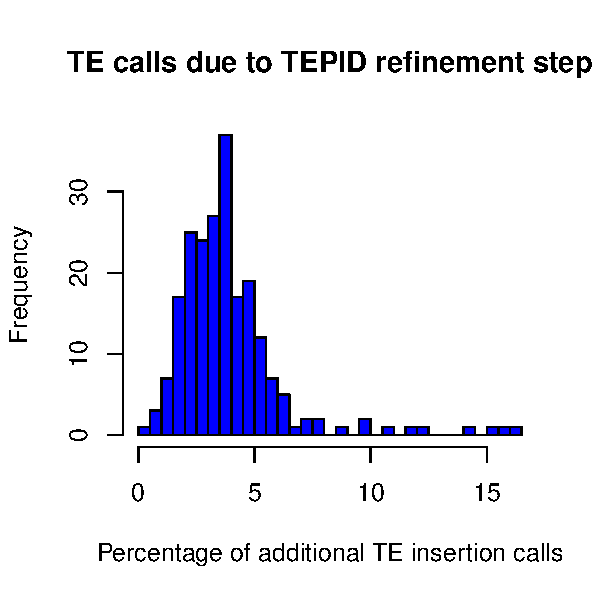
\includegraphics{Figure2/Figure2-figure_supplement_1.png}
  \caption{figure supplement 1}
  \label{fig2s1}
\end{suppfigure}

Percentage of total TE insertion calls that were made due to the TEPID
refinement step for each accession in the population.


\pagebreak
% Figure 2 - figure supplement 2
\setcounter{suppfigure}{1}

\begin{suppfigure}
  \centering
  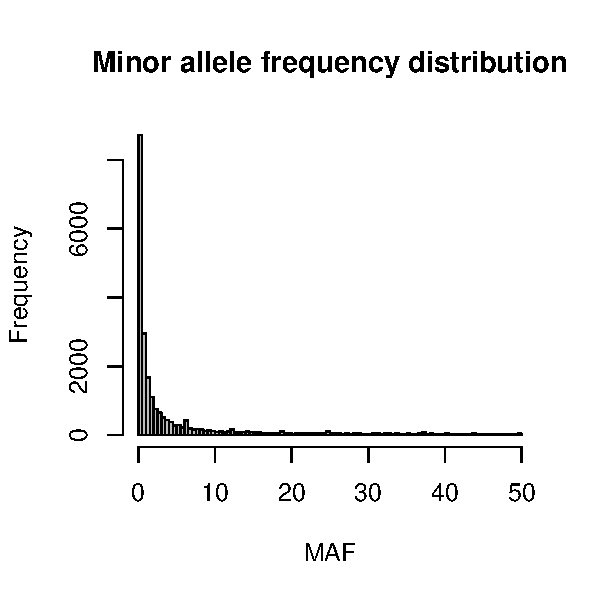
\includegraphics[width=0.5\textwidth]{Figure2/Figure2-figure_supplement_2.png}
  \caption{figure supplement 2}
  \label{fig2s2}
\end{suppfigure}

Number of accessions sharing TE variants identified by TEPID.

\pagebreak
% Figure 2 - figure supplement 3
\setcounter{suppfigure}{1}

\begin{suppfigure}
  \centering
  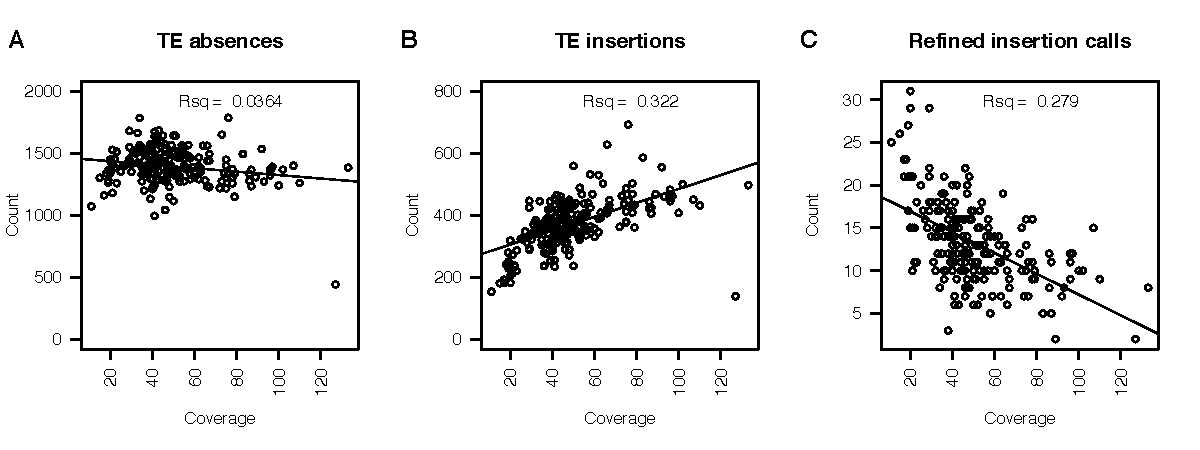
\includegraphics[width=1\textwidth]{Figure2/Figure2-figure_supplement_3.png}
  \caption{figure supplement 3}
  \label{fig2s3}
\end{suppfigure}

\begin{enumerate}
  \def\labelenumi{(\Alph{enumi})}
\item
  PCR validations for a TE absence variant. Accessions that were
  predicted to contain a TE insertion or TE absence are marked in bold.
  Two primer sets were used; forward (F) and reverse (R) or internal
  (I). Accessions with a TE absence will not produce the FI band and
  produce a shorter FR product, with the change in size matching the
  size of the deleted TE.
\item
  PCR validations for a TE insertion variant. One primer set was used,
  spanning the TE insertion site. A band shift of approximately 200 bp
  can be seen, corresponding to the size of the inserted TE.
\end{enumerate}

\pagebreak
% Figure 2 - figure supplement 4

\setcounter{suppfigure}{1}

\begin{suppfigure}
  \centering
  \includegraphics[width=1\textwidth]{Figure2/Figure2-figure_supplement_4.pdf}
  \caption{figure supplement 4}
  \label{fig2s4}
\end{suppfigure}

\begin{enumerate}
  \def\labelenumi{(\Alph{enumi})}
\item
  Number of TE absence variants identified versus the sequencing depth
  of coverage for each accession.
\item
  Number of TE insertion variants identified versus the sequencing depth
  of coverage for each accession.
\item
  Number of additional TE insertion calls made due to the TEPID
  refinement step versus sequencing depth of coverage for all
  accessions.
\end{enumerate}

\pagebreak
% Figure 2 - figure supplement 5
\setcounter{suppfigure}{1}

\begin{suppfigure}
  \centering
  \includegraphics[width=0.5\textwidth]{Figure2/Figure2-figure_supplement_5.png}
  \caption{figure supplement 5}
  \label{fig2s5}
\end{suppfigure}

Distribution of Type I and Type II elements over chromosome 1, for TE insertions and TE deletions.

\pagebreak
% Figure 2 - figure supplement 6

\setcounter{suppfigure}{1}

\begin{suppfigure}
  \centering
  \includegraphics[width=0.7\textwidth]{Figure2/Figure2-figure_supplement_6.png}
  \caption{figure supplement 6. Frequency of TE insertion in the \emph{KNOT} region}
  \label{fig2s6}
\end{suppfigure}

\begin{enumerate}
  \def\labelenumi{(\Alph{enumi})}
\item
  Number of TE insertion variants within each 300 kb \emph{KNOT ENGAGED ELEMENT (KEE)},
  vertical lines) and the number of TE insertion variants
  found in 10,000 randomly selected 300 kb windows (histogram).
\item
  Table showing number of TE insertion variants within each \emph{KEE}
  region, and the associated p-value determined by resampling 10,000
  times.
\end{enumerate}

\pagebreak

% Figure 2 - figure supplement 6
\setcounter{suppfigure}{1}

\begin{suppfigure}
  \centering
  \includegraphics[width=0.7\textwidth]{Figure2/Figure2-figure_supplement_7.png}
  \caption{figure supplement 7. Length distribution for all Col-0 TEs and all TE variants}
  \label{fig2s7}
\end{suppfigure}

\begin{enumerate}
  \def\labelenumi{(\Alph{enumi})}
\item
  Histogram showing lengths of all annotated TEs in the Col-0 reference
  genome.
\item
  Histogram showing lengths of all TE variants.
\item
  Density distribution of log10 TE length for all Col-0 TEs (red) and TE
  variants (blue).
\end{enumerate}

\pagebreak

% Figure 2 - figure supplement 7
\setcounter{suppfigure}{1}

\begin{suppfigure}[!ht]
  \centering
  \includegraphics[width=1\textwidth]{Figure2/Figure2-figure_supplement_8.png}
  \caption{figure supplement 8}
  \label{fig2s8}
\end{suppfigure}

TE family enrichments and depletions for TE insertions and TE deletions.

\pagebreak

% Figure 3

\begin{figure}[!ht]
  \centering
  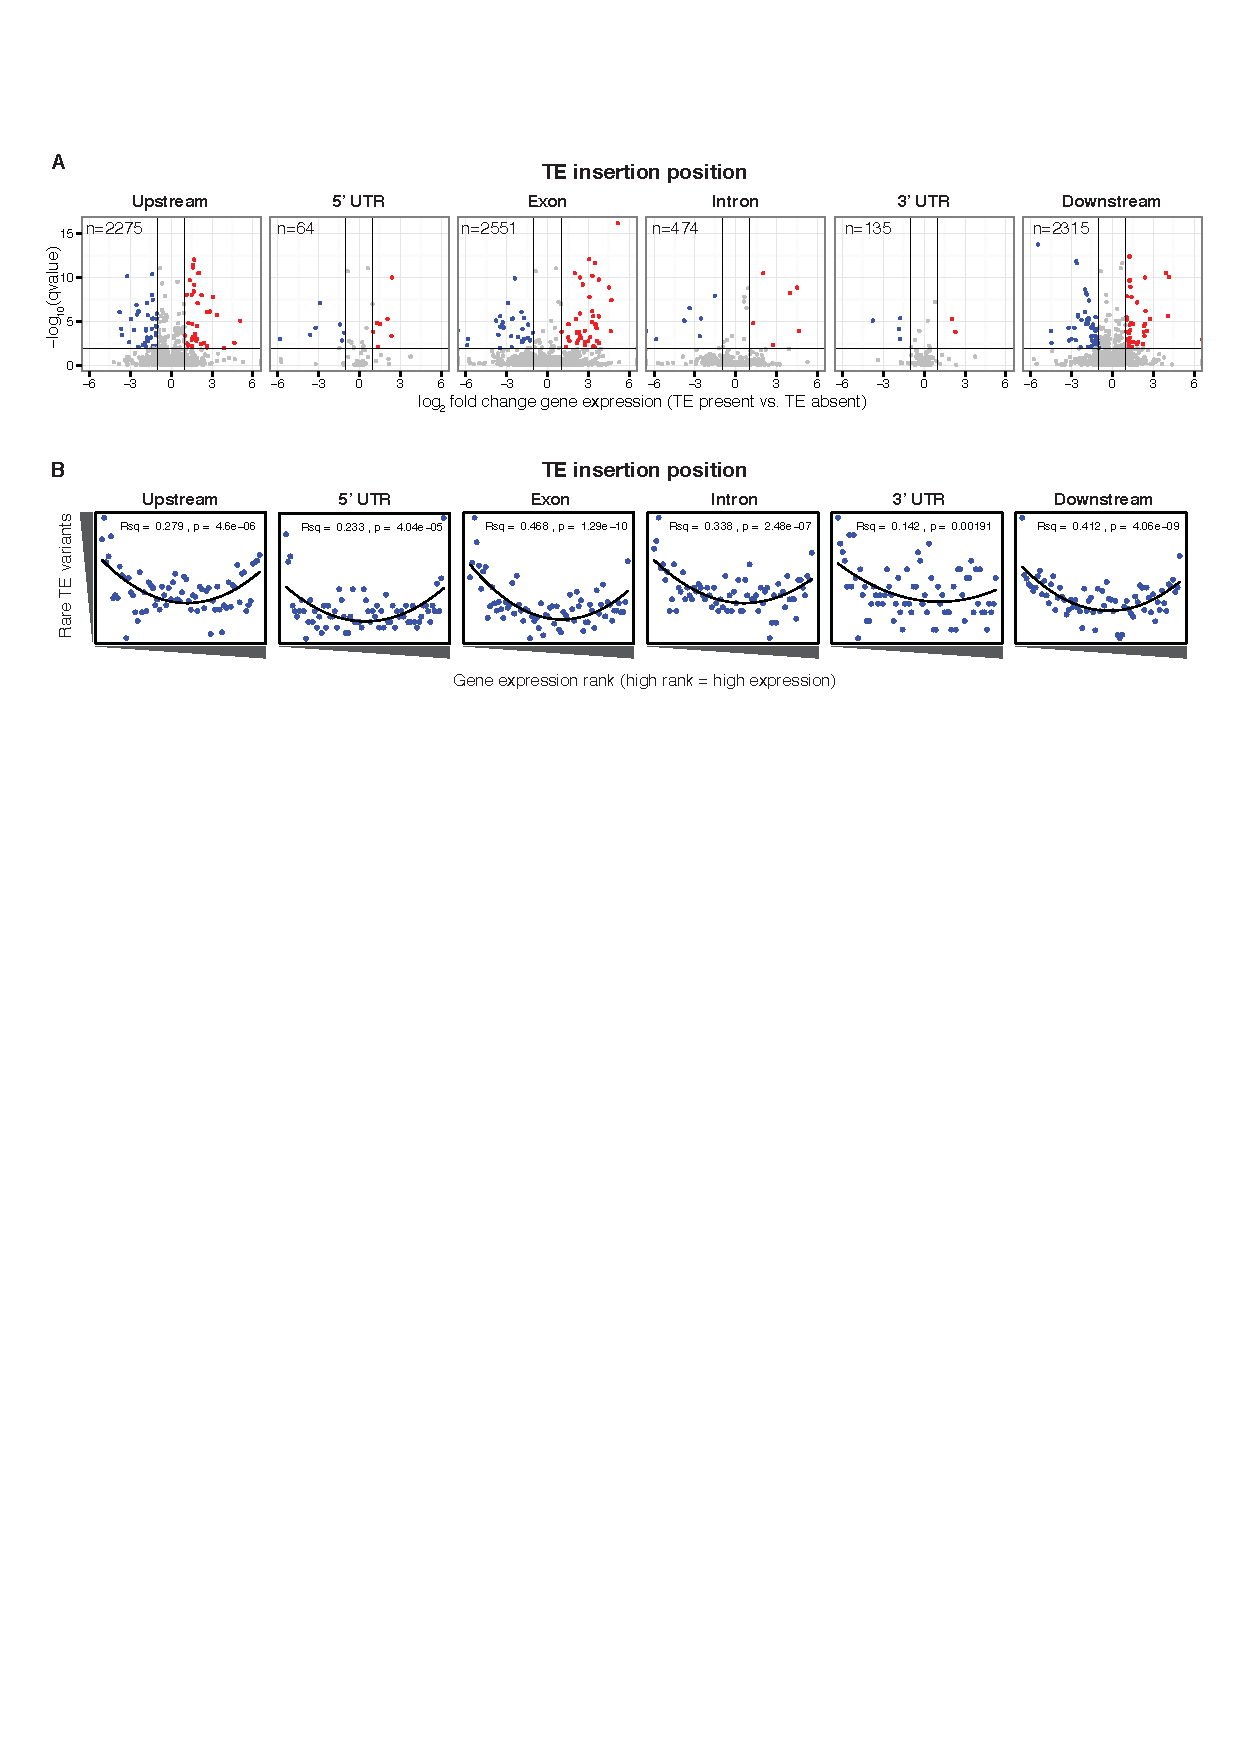
\includegraphics[width=0.5\textwidth]{Figure3/Figure3.png}
  \caption{Patterns of TE-SNP linkage}
  \label{fig3}
\end{figure}

\begin{enumerate}
  \def\labelenumi{(\Alph{enumi})}
\item
  r\textsuperscript{2} correlation matrices for individual representative high and low-LD
  TE variants showing the background level of SNP-SNP linkage.
\item
  Rank order plots for individual representative high and low-LD TE
  variants (matching those shown in A). Red line indicates the median r\textsuperscript{2}
  value for each rank across SNP-based values. Blue line indicates r\textsuperscript{2}
  values for TE-SNP comparisons. Grey lines indicate all individual
  SNP-SNP comparisons.
\item
  Histogram of the number of TE r\textsuperscript{2} ranks (0-600) that are above the
  SNP-based median r\textsuperscript{2} value for testable TE variants.
\item
  Boxplots showing distribution of minor allele frequencies for each LD
  category. Boxes represent the interquartile range (IQR) from quartile
  1 to quartile 3. Boxplot upper whiskers represent the maximum value,
  or the upper value of the quartile 3 plus 1.5 times the IQR (whichever
  is smaller). Boxplot lower whisker represents the minimum value, or
  the lower value of the quartile 1 minus 1.5 times the IQR (whichever
  is larger).
\end{enumerate}

(E). Proportion of TE insertions, TE deletions, and unclassified TE
variants in each LD category.

\pagebreak

% Figure 3 - figure supplement 1

\setcounter{suppfigure}{2}

\begin{suppfigure}
  \centering
  \includegraphics[width=0.7\textwidth]{Figure3/Figure3-figure_supplement1.png}
  \caption{figure supplement 1}
  \label{fig3s1}
\end{suppfigure}

Distribution of TE variants across chromosome 1 for each LD category
(high, mid, low).

\pagebreak

% Figure 4

\begin{figure}
  \centering
  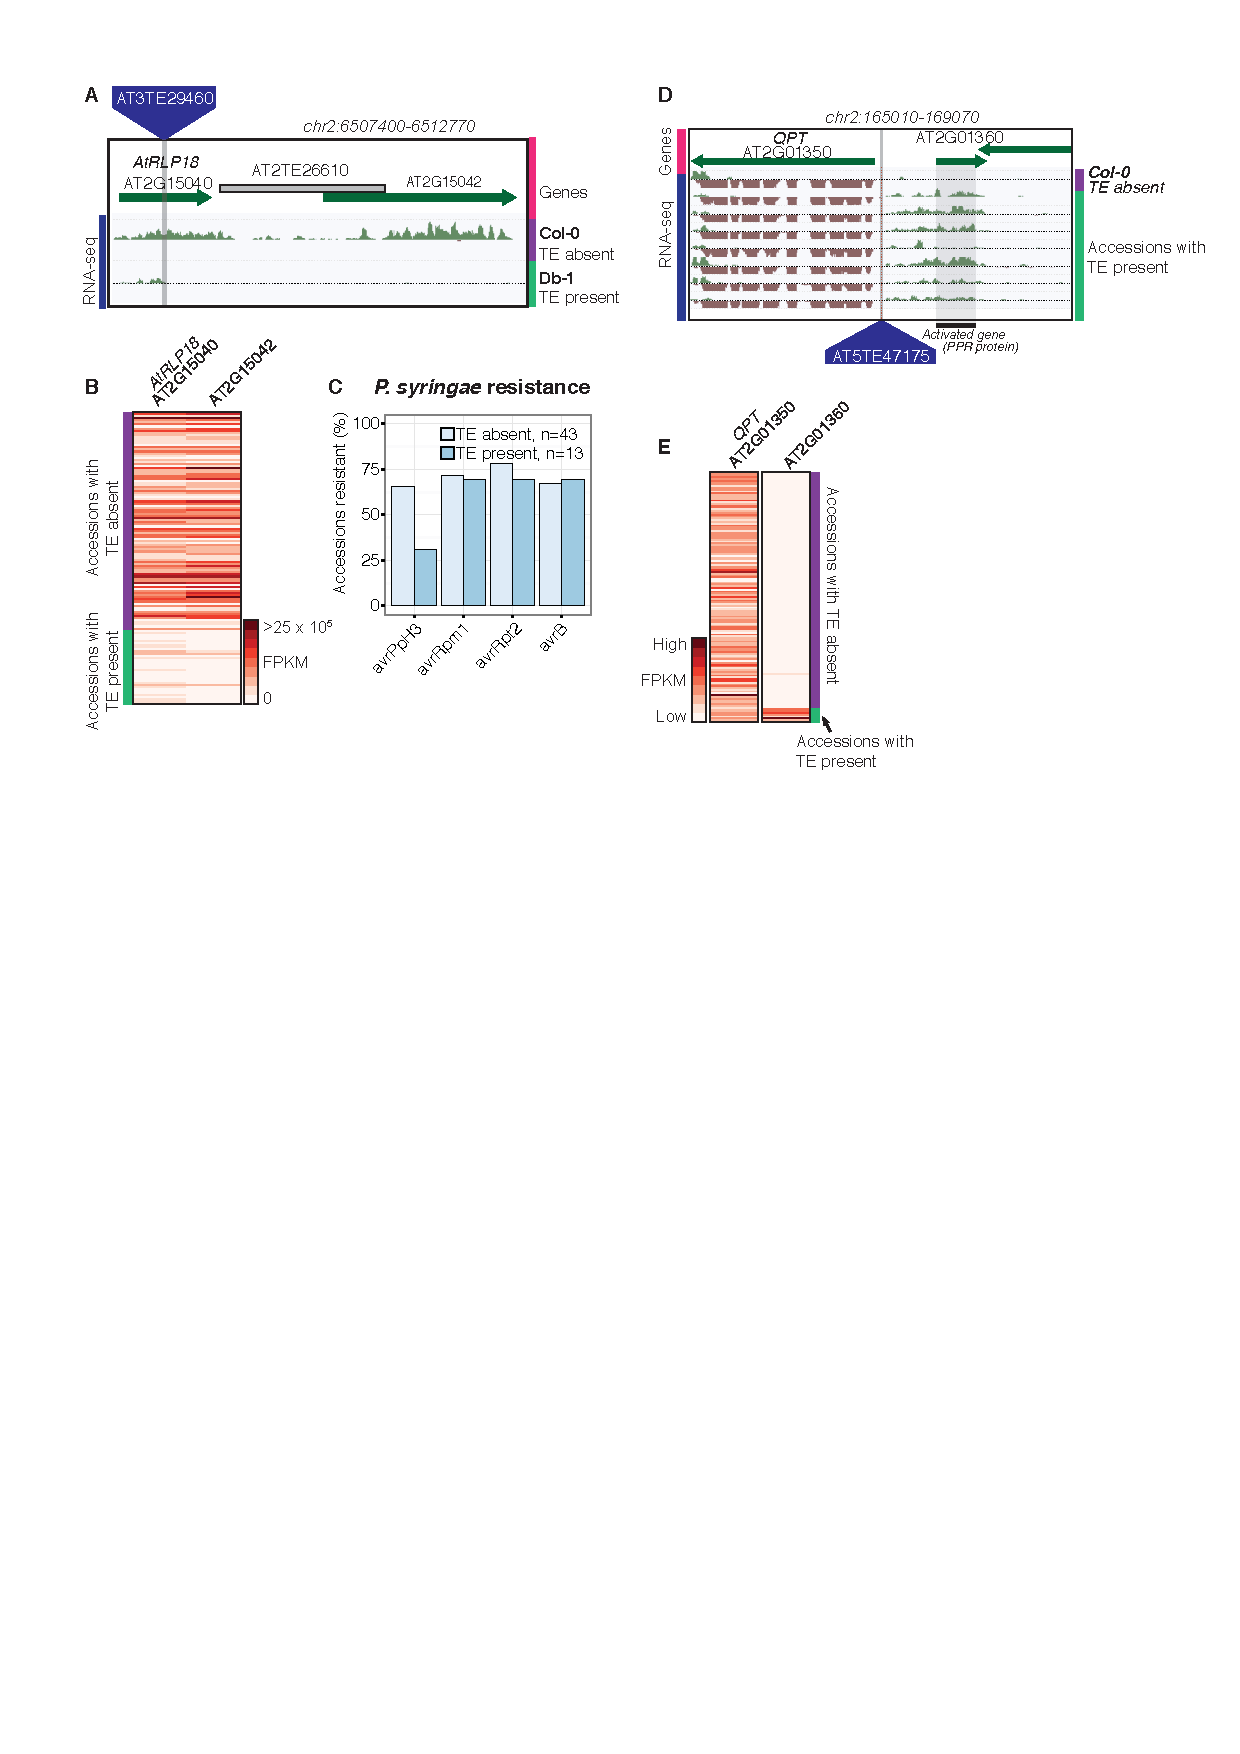
\includegraphics[width=1\textwidth]{Figure4/Figure4.png}
  \caption{Differential transcript abundance associated with TE variant presence/absence}
  \label{fig4}
\end{figure}

\begin{enumerate}
  \def\labelenumi{(\Alph{enumi})}
\item
  Volcano plots showing transcript abundance differences for genes
  associated with TE insertion variants at different positions,
  indicated in the plot titles. Genes with significantly different
  transcript abundance in accessions with a TE insertion compared to
  accessions without a TE insertion are colored blue (lower transcript
  abundance in accessions containing TE insertion) or red (higher
  transcript abundance in accessions containing TE insertion). Vertical
  lines indicate ±2 fold change in FPKM. Horizontal line indicates the
  1\% FDR.
\item
  Relationship between TE rare variant counts and gene expression rank.
  Plot shows the cumulative number of rare TE variants in equal-sized
  bins for gene expression ranks, from the lowest-ranked accession
  (left) to the highest-ranked accession (right). Lines indicate the fit
  of a quadratic model.
\end{enumerate}

\pagebreak

% Figure 4 - figure supplement 1

\setcounter{suppfigure}{3}

\begin{suppfigure}
  \centering
  \includegraphics[width=1\textwidth]{Figure4/Figure4-figure_supplement1.png}
  \caption{figure supplement 1}
  \label{fig4s1}
\end{suppfigure}

Relationship between rare TE variants and gene expression rank as for
Figure 4B, for permuted TE variants.

\pagebreak

% Figure 4 - figure supplement 2

\setcounter{suppfigure}{3}

\begin{suppfigure}
  \centering
  \includegraphics[width=1\textwidth]{Figure4/Figure4-figure_supplement2.png}
  \caption{figure supplement 2}
  \label{fig4s2}
\end{suppfigure}

Relationship between rare TE variants and gene expression rank as for
Figure 4B, for TE insertions (A) and TE deletions (B) separately.

\pagebreak

% Figure 5

\begin{figure}[!ht]
  \centering
  \includegraphics[width=0.8\textwidth]{Figure5/Figure5.png}
  \caption{Effects of TE variants on local gene expression}
  \label{fig5}
\end{figure}

\begin{enumerate}
  \def\labelenumi{(\Alph{enumi})}
\item
  Genome browser representation of RNA-seq data for genes \emph{AtRLP18}
  (AT2G15040) and a leucine-rich repeat family protein (AT2G15042) for
  Db-1, containing a TE insertion within the exon of the gene
  \emph{AtRLP18}, and for a Col-0 (not containing the TE insertion
  within the exon of \emph{AtRLP18}). Inset shows magnified view of the
  TE insertion site.
\item
  Heatmap showing \emph{AtRLP18 }and AT2G15042 RNA-seq FPKM values for
  all accessions.
\item
  Percentage of accessions with resistance to \emph{Pseudomonas syringae
  }transformed with different \emph{avr }genes, for accessions
  containing or not containing a TE insertion in \emph{AtRLP18}.
\item
  Genome browser representation of RNA-seq data for a PPR
  protein-encoding gene (AT2G01360) and \emph{QPT }(AT2G01350), showing
  transcript abundance for these genes in accessions containing a TE
  insertion variant in the upstream region of these genes.
\item
  Heatmap representation of RNA-seq FPKM values for \emph{QPT }and a
  gene encoding a PPR protein (AT2G01360), for all accessions. Note that
  scales are different for the two heatmaps, due to the higher
  transcript abundance of \emph{QPT} compared to AT2G01360. Scale
  maximum for AT2G01350 is $3.1\times10^5$, and for AT2G01360 is $5.9\times10^4$.
\end{enumerate}

\pagebreak

% Figure 6

\begin{figure}[!ht]
  \centering
  \includegraphics[width=0.8\textwidth]{Figure6/Figure6.png}
  \caption{TE variants are associated with nearby DMR methylation levels}
  \label{fig6}
\end{figure}


\begin{enumerate}
  \def\labelenumi{(\Alph{enumi})}
\item
  Distribution of distances from TE variants to the nearest population
  DMR, for TE deletions and TE insertions, C-DMRs and CG-DMRs.
\item
  Pearson correlation between DMR DNA methylation level and TE
  presence/absence, for all DMRs and their closest TE variant, versus
  the distance from the DMR to the TE variant (log scale). Blue lines
  show a linear regression between the correlation coefficients and the
  log10 distance to the TE variant.
\item
  Empirical cumulative distribution of Pearson correlation coefficients
  between TE presence/absence and DMR methylation level for TE
  insertions, TE deletions, C-DMRs and CG-DMRs. The Kolmogorov--Smirnov
  statistic is shown in each plot, indicated by \emph{D.}
\item
  Relationship between rare TE variant counts and nearby DMR DNA
  methylation level ranks, for TE insertions, deletions, C-DMRs, and
  CG-DMRs. Plot shows the cumulative number of rare TE variants in
  equal-sized bins of DMR methylation level ranks, from the lowest
  ranked accession (left) to the highest ranked accession (right). Lines
  indicate the fit of a quadratic model, and the corresponding R\textsuperscript{2} and p
  values are shown in each plot.
\end{enumerate}

\pagebreak

% Figure 6 - figure supplement 1

\setcounter{suppfigure}{5}

\begin{suppfigure}
  \centering
  \includegraphics[width=0.6\textwidth]{Figure6/Figure6-figure_supplement1.png}
  \caption{figure supplement 1}
  \label{fig6s1}
\end{suppfigure}

\begin{enumerate}
  \def\labelenumi{(\Alph{enumi})}
\item
  DNA methylation density distribution at C-DMRs within 1 kb of a TE
  variant (TE-DMRs) or further than 1 kb from a TE variant
  (non-TE-DMRs), in the presence or absence of the TE, for TE insertions
  and TE deletions.
\item
  As for A, for CG-DMRs.
\end{enumerate}


\pagebreak

% Figure 6 - figure supplement 2

\setcounter{suppfigure}{5}

\begin{suppfigure}
  \centering
  \includegraphics[width=0.5\textwidth]{Figure6/Figure6-figure_supplement2.png}
  \caption{figure supplement 2}
  \label{fig6s2}
\end{suppfigure}

Cumulative number DMR methylation level ranks for DMRs near rare TE
variants with accessions selected at random. Lines indicate the fit of a
quadratic model, and the corresponding R\textsuperscript{2} and p values are shown in each
plot.

\pagebreak

% Figure 6 - figure supplement 3

\setcounter{suppfigure}{5}

\begin{suppfigure}
  \centering
  \includegraphics[width=1\textwidth]{Figure6/Figure6-figure_supplement3.png}
  \caption{figure supplement 3}
  \label{fig6s3}
\end{suppfigure}

Selected examples of TE insertions apparently associated with
transcriptional downregulation of nearby genes and loss of gene body CG
methylation leading to the formation of a CG-DMR.

\pagebreak

% Figure 7

\begin{figure}
  \centering
  \includegraphics[width=1\textwidth]{Figure7/Figure7.png}
  \caption{Local patterns of DNA methylation surrounding TE variant sites}
  \label{fig7}
\end{figure}

\begin{enumerate}
  \def\labelenumi{(\Alph{enumi})}
\item
  Heatmap showing DNA methylation levels in 200 bp bins flanking TE
  variant sites, +/- 2 kb from the TE insertion point. TE variants were
  grouped into pericentromeric variants (\textless{}3 Mb from a
  centromere) or variants in the chromosome arms (\textgreater{}3 Mb
  from a centromere).
\item
  Line plot showing the DNA methylation level in each sequence context
  for TE insertion sites, +/- 2 kb from the TE insertion point.
\item
  As for B, for TE deletions.
\item
  Distribution of Pearson correlation coefficients between TE
  presence/absence and DNA methylation levels in the 200 bp regions
  flanking TE variant, ordered by distance to the centromere.
\end{enumerate}

\pagebreak

% Figure 7 - figure supplement 1

\setcounter{suppfigure}{6}

\begin{suppfigure}
  \centering
  \includegraphics[width=0.5\textwidth]{Figure7/Figure7-figure_supplement1.png}
  \caption{figure supplement 1}
  \label{fig7s1}
\end{suppfigure}

Heatmap showing DNA methylation levels in 200 bp bins flanking TE
variant sites in the 12 accessions with DNA methylation data for both
leaf and bud tissue, +/- 2 kb from the TE insertion point. TE variants
were grouped into pericentromeric variants (\textless{}3 Mb from a
centromere) or variants in the chromosome arms (\textgreater{}3 Mb from
a centromere).

\pagebreak

% Figure 8

\begin{figure}[!ht]
  \centering
  \includegraphics[width=0.5\textwidth]{Figure8/Figure8.png}
  \caption{Association scan between TE variants and C-DMR methylation variation}
  \label{fig8}
\end{figure}

\begin{enumerate}
  \def\labelenumi{(\Alph{enumi})}
\item
  Significant correlations between TE insertions and C-DMR DNA
  methylation level. Points show correlations between individual TE-DMR
  pairs that were more extreme than any of 500 permutations of the DMR
  data. Top plots show the total number of significant correlations for
  each TE insertion across the whole genome.
\item
  As for (A), for TE deletions.
\end{enumerate}

\pagebreak

\begin{table}[h]
  \centering
  \begin{threeparttable}
    \caption{Mapping of paired-end reads providing evidence for TE presence/absence
      variants in the L\emph{er} reference genome}
    \label{table1}
    \begin{tabular}{@{}cccccc@{}}
      \toprule
      \textbf{}  & \textbf{Concordant} & \textbf{Discordant} & \textbf{Split} & \textbf{Unmapped} & \textbf{Total} \\ \midrule
      Col-0 mapped & 0 & 993 & 9513 & 0 & 10206 \\
      L\emph{er} mapped & 10073 & 92 & 34 & 7 & 10206 \\ \bottomrule
    \end{tabular}
    \begin{tablenotes}
      \small
    \item Note: Discordant and split read categories are not mutually exclusive, as some discordant reads may have one read in the mate pair split-mapped.
    \end{tablenotes}
  \end{threeparttable}
\end{table}

\vspace*{1 cm}

\begin{table}[h]
  \centering
  \caption{Summary of TE variant classifications}
  \label{table2}
  \begin{tabular}{@{}ccc@{}}
    \toprule
    \textbf{TEPID call}        & \textbf{TE classification} & \textbf{Count} \\ \midrule
    \multirow{3}{*}{Insertion} & NA                         & 310            \\
    & Insertion                  & 14689          \\
    & Deletion                  & 8              \\ \midrule
    \multirow{3}{*}{Absence}   & NA                         & 1852           \\
    & Insertion                  & 388            \\
    & Deletion                   & 5848  \\ \bottomrule
  \end{tabular}
\end{table}

\vspace*{1 cm}

\begin{table}[h]
  \centering
  \caption{Percentage of DMRs within 1 kb of a TE variant}
  \label{table3}
  \begin{tabular}{@{}cccc|ccc@{}}
    \toprule
    \textbf{}              & \multicolumn{3}{c|}{\textbf{C-DMRs}}                     & \multicolumn{3}{c}{\textbf{CG-DMRs}}                    \\ \midrule
    \textbf{}              & \textbf{Observed} & \textbf{Expected} & \textbf{95\% CI} & \textbf{Observed} & \textbf{Expected} & \textbf{95\% CI} \\ \midrule
    \textbf{TE deletions}  & 17               & 16                & 0.0079           & 4.1               & 16                & 0.0041           \\
    \textbf{TE insertions} & 28                & 26                & 0.0089           & 9.1               & 26                & 0.0047           \\
    \textbf{NA calls}      & 8.7               & 6.2               & 0.0053           & 1.6               & 6.2               & 0.0027           \\
    \textbf{Total}         & 54                & 48                & 0.01             & 15                & 48                & 0.0054           \\ \bottomrule
  \end{tabular}
\end{table}

\end{document}
